\documentclass{article}%
\usepackage{amsmath}
\usepackage{amsfonts}
\usepackage{amssymb}
\usepackage{listings}
\usepackage{graphicx}
\usepackage{tikz}
\usepackage{multirow}
\usepackage{hyperref}%
\usepackage[a4paper,includeheadfoot,margin=0.5in]{geometry}
\setcounter{MaxMatrixCols}{30}
%TCIDATA{OutputFilter=late$x2$.dll}
%TCIDATA{Version=5.00.0.2552}
%TCIDATA{CSTFile=40 LaTeX article.cst}
%TCIDATA{Created=Thursday, August 21, 2008 14:03:59}
%TCIDATA{LastRevised=Wednesday, October 01, 2014 12:46:33}
%TCIDATA{<META NAME="GraphicsSave" CONTENT="32">}
%TCIDATA{<META NAME="SaveForMode" CONTENT="1">}
%TCIDATA{<META NAME="DocumentShell" CONTENT="Standard LaTeX\Blank - Standard LaTeX Article">}
%TCIDATA{Language=American English}
\newtheorem{theorem}{Theorem}
\newtheorem{acknowledgement}[theorem]{Acknowledgement}
\newtheorem{algorithm}[theorem]{Algorithm}
\newtheorem{axiom}[theorem]{Axiom}
\newtheorem{case}[theorem]{Case}
\newtheorem{claim}[theorem]{Claim}
\newtheorem{conclusion}[theorem]{Conclusion}
\newtheorem{condition}[theorem]{Condition}
\newtheorem{conjecture}[theorem]{Conjecture}
\newtheorem{corollary}[theorem]{Corollary}
\newtheorem{criterion}[theorem]{Criterion}
\newtheorem{definition}[theorem]{Definition}
\newtheorem{example}[theorem]{Example}
\newtheorem{exercise}[theorem]{Exercise}
\newtheorem{lemma}[theorem]{Lemma}
\newtheorem{notation}[theorem]{Notation}
\newtheorem{problem}[theorem]{Problem}
\newtheorem{proposition}[theorem]{Proposition}
\newtheorem{remark}[theorem]{Remark}
\newtheorem{solution}[theorem]{Solution}
\newtheorem{summary}[theorem]{Summary}
\newenvironment{proof}[1][Proof]{\noindent\textbf{#1.} }{\ \rule{0.5em}{0.5em}}

\usepackage{fancyhdr}
\setlength\headheight{26pt}
\pagestyle{fancy}
\lhead{{\footnotesize Assignment 3}}
\rhead{{\footnotesize Christopher Chapline}}
\begin{document}

\section*{Chapter 3}
\subsection*{Problem 36}
On the first network, the first 1004 data bytes will transmitted along with a 20 byte header and an offset of 0 for the
first message. For the second message, the remaining 20 data bytes, along with a 20 byte header will be transmitted. The
offset for this message will be 1004.\\
\\
On the second network, the first 556 data bytes with be transmitted along with the 20 byte header and an offset of 0. A
second message, containing the remaining 468 bytes along with a 20 byte header and an offset of 556.

\subsection*{Problem 46}
\subsubsection*{Part a}
\begin{tabular}{| c | l | l | l | l | l | l |}
    \hline
    \multirow{2}{*}{Information at node} &
    \multicolumn{6}{| c |}{Distance to reach node} \\ \cline{2-7}
      & A        & B        & C         & D        & E        & F        \\ \hline
    A & 0        & $\infty$ & 3         & 8        & $\infty$ & $\infty$ \\ \hline
    B & $\infty$ & 0        & $\infty$  & $\infty$ & 2        & $\infty$ \\ \hline
    C & 3        & $\infty$ & 0         & $\infty$ & 1        & 6        \\ \hline
    D & 8        & $\infty$ & $\infty$  & 0        & 2        & $\infty$ \\ \hline
    E & $\infty$ & 2        & 1         & 2        & 0        & $\infty$ \\ \hline
    F & $\infty$ & $\infty$ & 6         & $\infty$ & $\infty$ & 0        \\ \hline
\end{tabular}

\subsubsection*{Part b}
\begin{tabular}{| c | l | l | l | l | l | l |}
    \hline
    \multirow{2}{*}{Information at node} &
    \multicolumn{6}{| c |}{Distance to reach node} \\ \cline{2-7}
      & A        & B        & C         & D        & E        & F        \\ \hline
    A & 0        & $\infty$ & 3         & 8        & 10       & 9        \\ \hline
    B & $\infty$ & 0        & 3         & 4        & 2        & $\infty$ \\ \hline
    C & 3        & 3        & 0         & 3        & 1        & 6        \\ \hline
    D & 8        & 4        & 3         & 0        & 2        & $\infty$ \\ \hline
    E & 10       & 2        & 1         & 2        & 0        & 7        \\ \hline
    F & 9        & $\infty$ & 6         & $\infty$ & 7        & 0        \\ \hline
\end{tabular}

\subsubsection*{Part c}
\begin{tabular}{| c | l | l | l | l | l | l |}
    \hline
    \multirow{2}{*}{Information at node} &
    \multicolumn{6}{| c |}{Distance to reach node} \\ \cline{2-7}
      & A        & B        & C         & D        & E        & F        \\ \hline
    A & 0        & 6        & 3         & 8        & 10       & 9        \\ \hline
    B & 6        & 0        & 3         & 4        & 2        & 9        \\ \hline
    C & 3        & 3        & 0         & 3        & 1        & 6        \\ \hline
    D & 8        & 4        & 3         & 0        & 2        & 9        \\ \hline
    E & 10       & 2        & 1         & 2        & 0        & 7        \\ \hline
    F & 9        & 9        & 6         & 9        & 7        & 0        \\ \hline
\end{tabular}

\subsection*{Problem 52}
\begin{tikzpicture}[scale=0.2]
    \tikzstyle{every node}+=[inner sep=0pt]
    \draw [black] (18.7,-29.2) circle (3);
    \draw (18.7,-29.2) node {$A$};
    \draw [black] (26.7,-21.7) circle (3);
    \draw (26.7,-21.7) node {$B$};
    \draw [black] (41.3,-21.7) circle (3);
    \draw (41.3,-21.7) node {$C$};
    \draw [black] (26.7,-37.7) circle (3);
    \draw (26.7,-37.7) node {$D$};
    \draw [black] (41.3,-37.7) circle (3);
    \draw (41.3,-37.7) node {$E$};
    \draw [black] (50.9,-29.2) circle (3);
    \draw (50.9,-29.2) node {$F$};
    \draw [black] (20.89,-27.15) -- (24.51,-23.75);
    \fill [black] (24.51,-23.75) -- (23.59,-23.93) -- (24.27,-24.66);
    \draw [black] (24.51,-23.75) -- (20.89,-27.15);
    \fill [black] (20.89,-27.15) -- (21.81,-26.97) -- (21.13,-26.24);
    \draw [black] (20.76,-31.38) -- (24.64,-35.52);
    \fill [black] (24.64,-35.52) -- (24.46,-34.59) -- (23.73,-35.28);
    \draw [black] (24.64,-35.52) -- (20.76,-31.38);
    \fill [black] (20.76,-31.38) -- (20.94,-32.31) -- (21.67,-31.62);
    \draw [black] (29.7,-37.7) -- (38.3,-37.7);
    \fill [black] (38.3,-37.7) -- (37.5,-37.2) -- (37.5,-38.2);
    \draw [black] (38.3,-37.7) -- (29.7,-37.7);
    \fill [black] (29.7,-37.7) -- (30.5,-38.2) -- (30.5,-37.2);
    \draw [black] (29.7,-21.7) -- (38.3,-21.7);
    \fill [black] (38.3,-21.7) -- (37.5,-21.2) -- (37.5,-22.2);
    \draw [black] (38.3,-21.7) -- (29.7,-21.7);
    \fill [black] (29.7,-21.7) -- (30.5,-22.2) -- (30.5,-21.2);
    \draw [black] (48.54,-27.35) -- (43.66,-23.55);
    \fill [black] (43.66,-23.55) -- (43.99,-24.43) -- (44.6,-23.65);
    \draw [black] (43.66,-23.55) -- (48.54,-27.35);
    \fill [black] (48.54,-27.35) -- (48.21,-26.47) -- (47.6,-27.25);
    \draw [black] (48.65,-31.19) -- (43.55,-35.71);
    \fill [black] (43.55,-35.71) -- (44.48,-35.56) -- (43.81,-34.81);
    \draw [black] (43.55,-35.71) -- (48.65,-31.19);
    \fill [black] (48.65,-31.19) -- (47.72,-31.34) -- (48.39,-32.09);
\end{tikzpicture}

\subsection*{Problem 55}
\subsubsection*{Part a}
This packet will be directly delivered over \textbf{interface 0}.
\subsubsection*{Part b}
This packet will be forwarded to \textbf{R2}.
\subsubsection*{Part c}
This packet will be forwarded to \textbf{R4}
\subsubsection*{Part d}
This packet will be forwarded to \textbf{R3}
\subsubsection*{Part e}
This packet will be forwarded to \textbf{R4}

\subsection*{Problem 64}
\subsubsection*{Part a}
This could happen if A's message was sent before the A-B link was restored
or if B's message was sent before the A-B link was severed.
\subsubsection*{Part b}
C should assume that the A-B link is down until it receives another message from A saying
that the link has been restored.

\end{document}
